\documentclass[journal]{IEEEtran}
\usepackage{amsmath,amsfonts}
\usepackage{algorithmic}
\usepackage{algorithm}
\usepackage{array}
\usepackage[caption=false,font=normalsize,labelfont=sf,textfont=sf]{subfig}
\usepackage{textcomp}
\usepackage{stfloats}
\usepackage{url}
\usepackage{verbatim}
\usepackage{graphicx}
\usepackage{cite}
\usepackage[spanish]{babel}
\usepackage{tikz}

\usepackage{bookmark}

\hyphenation{op-tical net-works semi-conduc-tor IEEE-Xplore}
% updated with editorial comments 8/9/2021
\begin{document}

\title{Evaluación de algoritmos de búsqueda para la resolución del problema de las jarras}

\author{\IEEEauthorblockN{Edson Elias Reza Garduño}}

\maketitle

\begin{abstract}
  El problema de las jarras es un clásico ejemplo de un problema matemático y lógico que requiere de habilidades de razonamiento y pensamiento creativo para resolverlo. Resolver este problema puede tener aplicaciones prácticas en el campo de la inteligencia artificial, la optimización y la resolución de problemas, lo que lo hace un tema de gran interés en la investigación y el aprendizaje. En esta ocasion se propone la implementación de algoritmos de búsqueda para resolver dicho problema.
\end{abstract}

\section{Introducción}
Sean dos jarras de capacidad $x$ y $y$ respectivamente, y un líquido de capacidad infinita. Se desea obtener $z$ litros de líquido en una de las jarras. ¿Cómo se puede lograr esto?.

El enunciado anterior es la descripción del problema de las jarras, un problema clásico que se puede encontrar en libros de matemáticas, en la literatura de inteligencia artificial y en la web. El problema de las jarras es un problema de búsqueda en el que se busca una solución a un problema a partir de un estado inicial. En este caso, el estado inicial es el estado en el que se encuentran las jarras, y el estado final es el estado en el que se encuentran las jarras después de haber realizado las operaciones necesarias para obtener $z$ litros de líquido en una de las jarras.

Para lograr alcanzar $z$ se consideran algunas restricciones:
\begin{itemize}
  \item No se puede medir el líquido que se encuentra en las jarras, solo se puede saber si la jarra está vacía o llena, asi como la cantidad restante de alguna operación.
  \item Solo se pueden realizar las siguientes operaciones:
        \begin{itemize}
          \item Llenar la jarra de $x$ litros.
          \item Llenar la jarra de $y$ litros.
          \item Vaciar la jarra de $x$ litros.
          \item Vaciar la jarra de $y$ litros.
          \item Llenar la jarra de $x$ litros desde la jarra de $y$ litros.
          \item Llenar la jarra de $y$ litros desde la jarra de $x$ litros.
        \end{itemize}
\end{itemize}

Viendo el problema, se puede obtener la solución rápida y fácilmente, sin embargo, para el caso de que se desee obtener la solución de manera automática, la solución para la computadora no es tan evidente.
Después de todo, la computadora no puede pensar como un humano, por lo que se requiere de un algoritmo que le indique a la computadora qué operaciones realizar para llegar a la solución.
Pero ahora tenemos otro problema, ¿cómo se puede implementar un algoritmo que le indique a la computadora qué operaciones realizar para llegar a la solución?. Es en este punto cuando aparecen los algoritmos de búsqueda, que son algoritmos que permiten encontrar una solución a un problema a partir de un estado inicial. Aun así, cabe mencionar que este problema puede ser resuelto de muchas otras maneras, pero nos enfocaremos en los algoritmos de búsqueda.

Considerado solo dos jarras, la complejidad de este problema se puede aproximar como $O(m \cdot n)$, donde $m$ y $n$ son las capacidades de cada jarra. La cantidad de estados aumenta como se muestra a continuación:

\begin{figure}[h]
  \centering
  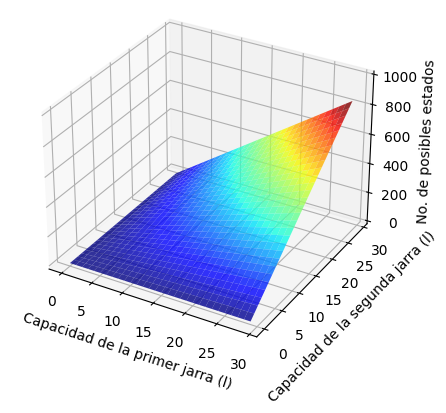
\includegraphics[width=0.45\textwidth]{figures/estados.png}
  \centering
  \caption{Cantidad de estados}
  \label{fig:estados}
\end{figure}

En la figura \ref{fig:estados} se puede observar la cantidad de estados posibles y como aumentan en función de las capacidades de las jarras. Es importante recordar que no todos los posibles estados son alacanzables, por lo que la cantidad de estados alcanzables es menor a la cantidad de estados totales.

En este trabajo, usaremos algunos algorimos de búsqueda para resolver el problema de las jarras, comparando los resultados obtenidos entre si, a fin de determinar cuales son los algoritmos más eficientes para resolver este problema.
\section{Trabajos relacionados}

\section{Enfoque}
Formulamos el problema de las jarras como un árbol de búsqueda, donde cada nodo representa un estado, y cada arista representa una operación. Como muchos de este tipo de problemas, varias veces una operación puede llevar a un estado que ya se ha visitado, por lo que se debe de tener cuidado de no repetir estados.
Para lograr eso ultimo, existirá una lista de estados visitados, y cada vez que se visite un estado, se revisará si ya se ha visitado, en caso de que ya se haya visitado, se ignorará el estado, evitando así desarrollos infinitos.

Para cada nodo se podrán desarrollar hasta 6 hijos, uno para cada operación, a consideración de que la operación sea posible de realizar. Por ejemplo, si la jarra de $x$ litros está llena, no se podrá realizar la operación de llenar la jarra de $x$ litros, ya que la jarra ya está llena. Por otro lado, si la jarra de $y$ litros está vacía, no se podrá realizar la operación de vaciar la jarra de $y$ litros, ya que la jarra ya está vacía. Para estos casos, se ignorará la operación, y se desarrollará el siguiente hijo.
Y siempre teniendo en consideración que el estado final deseado puede no ser alcanzable.

\begin{figure}[h]
  \centering
  \scalebox{0.6}{
    \begin{tikzpicture}[level distance=2cm,
        level 1/.style={sibling distance=6cm},
        level 2/.style={sibling distance=3cm}]
      \node[circle,draw] (root) {$(0,0)$}
      child {
          node[circle,draw] {$(4,0)$}
          child {
              node[circle,draw] {$(1,3)$}
              child {node[circle,draw] {$(1,0)$}}
              child {node[circle,draw] {$(4,3)$}}
            }
          child {
              node[circle,draw] {$(0,4)$}
              child {node[circle,draw] {$(4,4)$}}
              child {node[circle,draw] {$(1,3)$}}
            }
        }
      child {
          node[circle,draw] {$(0,3)$}
          child {
              node[circle,draw] {$(3,0)$}
              child {node[circle,draw] {$(3,3)$}}
              child {node[circle,draw] {$(0,0)$}}
            }
          child {
              node[circle,draw] {$(0,3)$}
              child {node[circle,draw] {$(3,3)$}}
              child {node[circle,draw] {$(0,0)$}}
            }
        };

    \end{tikzpicture}
  }
  \caption{Árbol de los estados de las jarras}
  \label{fig:arbol}
\end{figure}

Como se puede observar en la figura \ref{fig:arbol}, el árbol de búsqueda puede generar recursiones, y algunos estados se pueden alcanzar por más de una manera, de ahí la importancia de tener una estructura de datos que permita almacenar los estados visitados, para evitar desarrollos infinitos.

Con el problema ya planteado, se puede proceder a implementar los algoritmos de búsqueda, y comparar los resultados obtenidos entre si. Para este trabajo, se implementarán los siguientes algoritmos de búsqueda:

\subsection{Búsqueda en amplitud}
El algoritmo de búsqueda en amplitud es un algoritmo de búsqueda no informada, que consiste en desarrollar los nodos de un árbol de búsqueda en amplitud, es decir, primero se desarrollan los nodos del nivel 1, después los del nivel 2, y así sucesivamente. Este algoritmo es muy sencillo de implementar, pero no es muy eficiente, ya que puede tardar mucho tiempo en encontrar la solución, y puede requerir mucha memoria para almacenar los nodos desarrollados.
Pero a pesar de su alto costo, nos da la garantía de encontrar la solución más corta (si es que existe).

\subsection{Búsqueda en profundidad}
El algoritmo de búsqueda en profundidad es un algoritmo de búsqueda no informada, que consiste en desarrollar los nodos de un árbol de búsqueda en profundidad, es decir, primero se desarrollan los nodos del nivel más profundo, después los del nivel anterior, y así sucesivamente. Al igual que el anterior este tambien es muy sencillo de implementar, pero no siempre va a encontrar la solución más óptima, pues si encuentra una solución valida, se detiene, y no sigue desarrollando el árbol, evitando que pueda descubrir una mejor solución en otra rama del árbol.

\subsection{Búsqueda en profundidad limitada}
El algoritmo de búsqueda en profundidad limitada es una variante del algoritmo de búsqueda en profundidad, que consiste en desarrollar los nodos de un árbol de búsqueda en profundidad, pero limitando la profundidad a la que se desarrolla el árbol. Este algoritmo es muy útil cuando se desconoce la profundidad del árbol, y se desea encontrar una solución en un tiempo razonable. Con la limitación se puede mejorar además del tiempo de ejecución, el espacio de memoria requerido y se puede llegar a mejorar la solución encontrada. Como desventaja, al limitar la profundidad, se puede llegar a no encontrar alguna solución, pues esta puede estar más profundo en el árbol.

\subsection{Búsqueda en profundidad iterativa}
El algoritmo de búsqueda en profundidad iterativa es una variante del algoritmo de búsqueda en profundidad, que consiste en desarrollar los nodos de un árbol de búsqueda en profundidad, pero limitando la profundidad a la que se desarrolla el árbol, y aumentando la profundidad en cada iteración en caso de que no se haya podido encontrar una solución. El algoritmo cumple en menor medida con las mismas ventajas que el algoritmo de búsqueda en profundidad limitada, pero al aumentar la profundidad en cada iteración, nos aseguramos de encontrar una solución, aunque no sea la más óptima, y si es que existe. Como desventaja mayor esta el hecho de que cada incremento implica volver a desarrollar el árbol, por lo que el tiempo de ejecución aumenta considerablemente si la profundidad se empieza a incrementar mucho.

\subsection{Búsqueda voraz}
O greedy, es un algoritmo de busqueda informada, que consiste en desarrollar los nodos de un árbol de búsqueda, pero en cada paso se elige el nodo que tenga el menor costo basado en una función heurística. Su mayor limitante será la calidad de la función heurística, pues si esta no es buena, el algoritmo no podrá encontrar una solución óptima.

\subsection{Búsqueda A*}
El algoritmo A* es un algoritmo de búsqueda informada, que consiste en desarrollar los nodos de un árbol de búsqueda, pero en cada paso se elige el nodo que tenga el menor costo basado en una función heurística, y el costo acumulado hasta ese nodo. Al igual que la búsqueda voraz, su mayor limitante será la calidad de la función heurística, junto con el costo acumulado. Con el uso de estos dos factores, si bien no se garantiza encontrar la solución más óptima, se puede asegurar que la solución encontrada será ``buena'' en terminos de costo.

\section{Experimentación}
Se implementó un programa en Python que permite utilizar dos jarras y una lista de estados objetivo.
Tanto la capacidad de las jarras como la lista de estados objetivo se pueden modificar en el archivo \textit{main.py}, en la función \textit{main}.

Con los estados recibidos, se ejecutan todos los algoritmos de búsqueda, y se imprime en pantalla la cantidad de nodos desarrollados por cada uno hasta alcanzar una solución, o hasta que se agote el espacio de búsqueda. Tambien muestra el camino que se debe seguir para llegar a la solución si es que se encontró una.

En esta ocasión el parametro que se usó para comparar los algoritmos fue la cantidad de nodos desarrollados, ya que es un parámetro que se puede medir fácilmente, y que nos da una idea de la eficiencia de cada algoritmo al momento de encontrar una solución.

\section{Conclusion}
De todos los algoritmos de búsqueda implementados, el que peor desempeño tuvo fue la búsqueda en profundidad iterativa, pues si no se encontraba la solución en la primera iteración, la cantidad de nodos desarrollados aumentaba considerablemente en cada iteración. La búsqueda en amplitud sin duda siempre daba la respuesta más eficiente, como se esperaba, pero si la solución estaba en una parte profunda del árbol, podia desarrollar demasiados nodos. Si de antemano se conoce por donde se encuentra la solución la búsqueda en profundidad limitada es la mejor opción, pues se puede limitar la profundidad y lograr conseguir una solución lo suficientemente buena en un tiempo razonable. La búsqueda voraz y A* son algoritmos muy similares, pues ambos utilizan una función heurística para decidir cual es el siguiente nodo a desarrollar, pero A* utiliza el costo acumulado hasta ese nodo, lo que le da una ventaja sobre la búsqueda voraz, pues si bien no se garantiza encontrar la solución más óptima, se puede asegurar que la solución encontrada será ``buena'' con mayor seguridad respecto al resto de algorimos.

\section{Trabajos futuros}
Es posible generalizar el problema para que se pueda utilizar un número arbitrario de jarras, por lo que se puede implementar para conocer si los resultados vistos en este trabajo se mantienen, o por el contrario, cambian conforme se aumenta el número de jarras, y si es así, observar como cambian los resultados de los algoritmos de búsqueda.
Tambien se puede explorar el uso de los algoritmos vistos en problemas similares, donde se tengan recursos de almacenamiento limitado.
De manera secundaria, se pueden explorar medios para mejorar el rendimiento de los algoritmos sin cambiar su lógica de funcionamiento, como por ejemplo, implementarlos en lenguajes de programación compilados, o utilizando paralelismo para recorrer el árbol de búsqueda más rápido.

\begin{thebibliography}{1}
  \bibliographystyle{IEEEtran}

  \bibitem{ref1}M. S. Gupta and S. Bairagi, {\it{“Evaluating Search Algorithms for Solving n-Puzzle”,}} [Online]. Available: http://sumitg.com/assets/n-puzzle.pdf

  \bibitem{ref2}H. Franco, {\it{“Búsqueda no informada Métodos en anchura y de costo uniforme”,}} [Online]. Available: https://hpclab.ucentral.edu.co/wp-content/uploads/2021/09/Session\_8\_UninformedSearch.pdf

\end{thebibliography}

\end{document}


